
% !TEX encoding = ISO-8859-1

Os dados gerados para serem analisados nos experimentos foram especificados como um conjunto de 300 padrões formando 3 conjuntos, um conjunto com 150 padrões, outro com 100 e a última com 50 padrões. Esses padrões são descritos por duas variáveis quantitativas, e todos gerados a partir de distribuições bi-variadas, conforme a tabela \ref{tab:dados}.

\begin{table}[H]
\begin{center}
\begin{tabular}{|l|l|l|l|l|l|l|l|}
\hline
Conjunto 				& 	Classe	&	$\mu_1$	&	$\mu_2$	&	$\sigma_1$	&	$\sigma_2$	&	$\sigma_{12}$	&	$\rho_{12}$	\\
\hline %----- linha horizontal
Conjunto 1           	&	1		&   0.00   	&   0.00    &   	2   	&		1   	&		1.7		&		0.85	\\
Conjunto 2     			&   2		&   0.00	&   3		&   	0.5		&   	0.5   	&		0.00	&		0.00	\\
Conjunto 3     			&   2		&   4		&   3		&   	2		&   	1   	&		-1.7	&		-0.85	\\
\hline
\end{tabular}%--- fechamento do ambiente tabular
\end{center}   %fim da centralização da tabela
\caption{Dados para geração do conjunto de padrões}
\label{tab:dados}
\end{table}

Para criar os conjuntos com os dados acima, foi utilizada a função do matlab $mvnrnd(\mu, \sigma, q)$, sendo $q$ a quantidade de instâncias a serem geradas. Os dados gerados formam um conjunto muito próximo do ideal, citado acima, por isso, considera-se que os padrões obedecem totalmente aos dados acima.

\begin{figure}[H]
\center
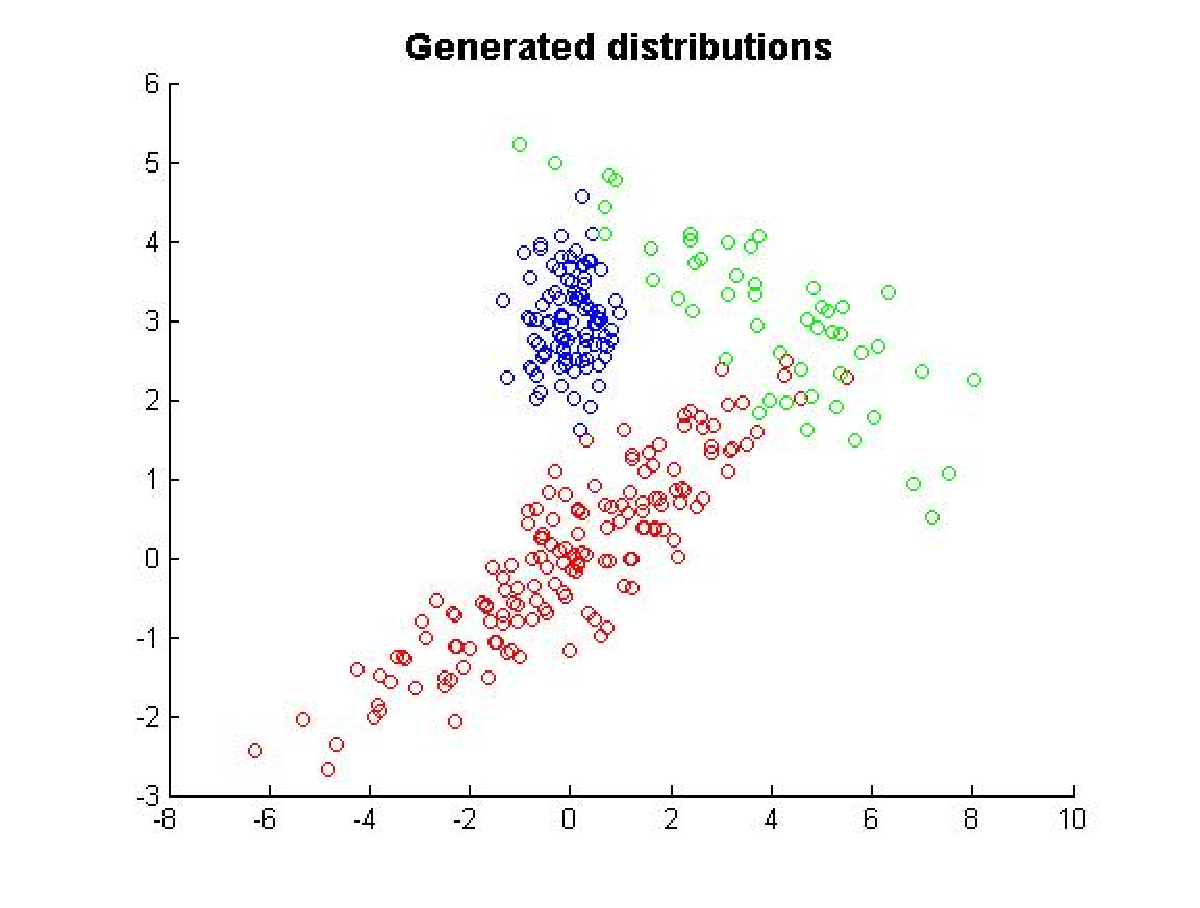
\includegraphics[scale=0.60]{imagens/tecnicas/generatedDistributions.eps}
\caption{Dados gerados para os experimentos}
\label{fig:dados}
\end{figure}


A figura \ref{fig:dados} mostra o resultado final da base de dados gerada. Este conjunto resultante será o referencial para todos os experimentos que seguem.
